\section{Subprogramas en VHDL: Funciones y procedimientos \label{sec:s1}}

\begin{center}
	\begin{minipage}{12cm}
		\begin{tcolorbox}[title=Actividad 1]
			Capturar los códigos escritos en VHDL vistos en clase, compilarlos y simularlos (se proporcionan en la presentación y en el documento anexo). Ver el resultado de la síntesis con el visor RTL.
		\end{tcolorbox}	
	\end{minipage}
\end{center}

La visualización RTL de los 3 sumadores de 4 bits en VHDL se muestra en la \autoref{fig:subprogram_3_adders_rtl_vhdl}. Como se observa, la implementación se realiza utilizando 3 instancias de sumadores de 4 bits, independientes una de otra. Las simulaciones se visualizan en la \autoref{fig:subprogram_3_adders_wavebi_vhdl} en base binaria y en la \autoref{fig:subprogram_3_adders_wavede_vhdl} en base decimal, en donde se muestra que la suma se hace de manera correcta en cada elemento.

En los Anexos se localiza la descripción de los 3 sumadores de 4 bits. Las 3 implementaciones comparten la misma declaración de bibliotecas y de entidad, difiriendo en la definición de la arquitectura.

\begin{itemize}
	\item \textbf{Para el caso de la función:} Se genera el prototipo y la cabecera de la función, declarando dos parámetros que servirán como operadores de apoyo para la suma (Op1 y Op2) y una variable que devolverá la función como resultado (Total). En el cuerpo de la función se realiza la suma de los dos operandos y se asigna con ``:='' el resultado a la variable que se va a retornar. Finalmente, en el cuerpo de la arquitectura se llama a la función, dándole los parámetros necesarios y asignando con ``$<$='' el resultado a la señal correspondiente.
	\item \textbf{Para el caso del procedimiento (caso 1):} Se genera el prototipo y la cabecera del procedimiento, declarando tres parámetros, dos de ellos serán las entradas que sirven como operadores de apoyo para la suma (Op1 y Op2) y otra variable que será la salida que almacena el resultado (Total). En el cuerpo del procedimiento unicamente se realiza la suma, asignando con ``:='' el resultado. Finalmente, en el cuerpo de la arquitectura se declaran tanto una lista sensible para las entradas como las variables en donde se guardará el resultado de cada suma. Dentro del bloque \textit{process} se llaman a los procedimientos para después asignar a las señales de salida el valor de las variables declaradas previamente (usando ``$<$='').
	\item \textbf{Para el caso del procedimiento (caso 2):} Es muy parecido al caso 1, solo que en el prototipo y cabecera del procedimiento se declara a la salida como señal. Esto provoca que en el cuerpo del procedimiento se use ``$<$='' para asignar el resultado y en el cuerpo de la arquitectura desaparece la lista sensible y la declaración de variables, haciendo que solo se llame al procedimiento, colocando a las señales como parámetros.
\end{itemize}

\begin{figure}[ht]
	\centering
	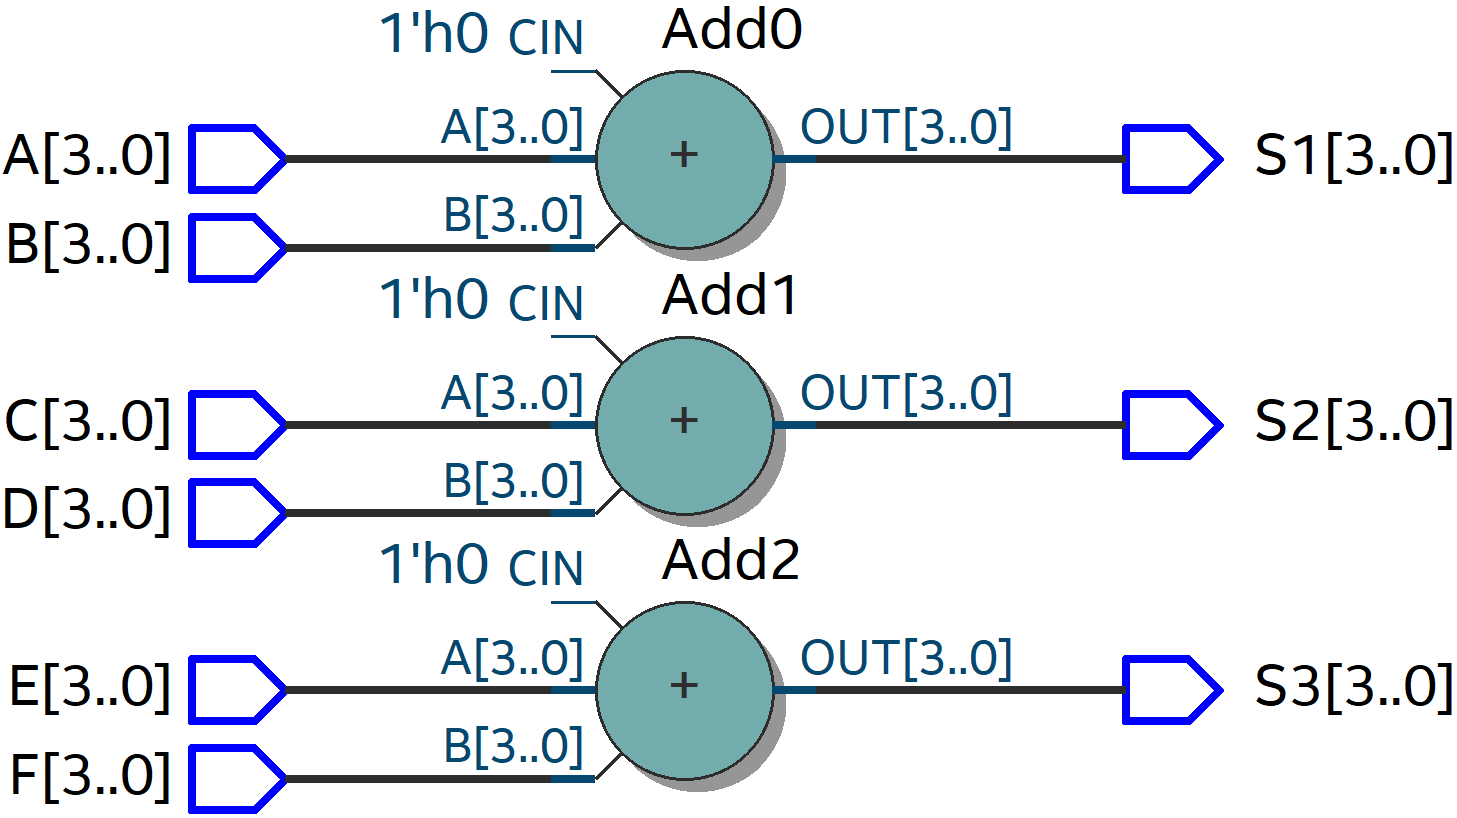
\includegraphics[scale=0.43]{Subprogram_3_Adders_RTL.png}
	\caption{Diagrama RTL de los 3 sumadores de 4 bits implementados en VHDL. Se tiene el mismo resultado si se usan funciones o procedimientos. \label{fig:subprogram_3_adders_rtl_vhdl}}
\end{figure}

\begin{figure}[ht]
	\centering
	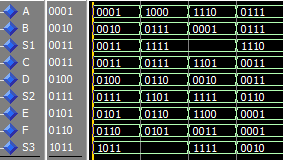
\includegraphics[scale=1.5]{Subprogram_3_Adders_WaveBi.png}
	\caption{Simulación de los 3 sumadores de 4 bits con el visor de formas de onda de ModelSim (base binaria). \label{fig:subprogram_3_adders_wavebi_vhdl}}
\end{figure}

\begin{figure}[ht]
	\centering
	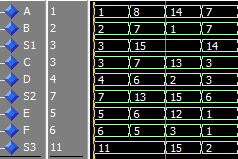
\includegraphics[scale=1.5]{Subprogram_3_Adders_WaveDe.png}
	\caption{Simulación de los 3 sumadores de 4 bits con el visor de formas de onda de ModelSim (base decimal). \label{fig:subprogram_3_adders_wavede_vhdl}}
\end{figure}